% !TEX root = ../main.tex
\section{Validação de Resultados e Análise Comparativa}
\label{sec:validacao}

A validação física, numérica e estatística do pipeline desenvolvido em 2026 estruturou-se em quatro vertentes complementares: (i) confronto teórico com as correlações consensuais de fluxo de deriva (\emph{drift-flux}) na literatura internacional, (ii) análise da evolução temporal da fração de vazio instantânea $\alpha(t)$ em séries contínuas a alta velocidade, (iii) comparação direta entre a nova formulação de duplo regime em Python e o método voxelizado prévio em MATLAB, e (iv) aplicação do algoritmo à base de dados experimental de referência em minicanais.

\subsection{Confronto com a Teoria de Deriva de Rouhani--Axelsson}
\label{subsec:validacao_rouhani}

No estudo de escoamentos bifásicos ebulitivos em condutas circulares, a correlação analítica de maior consenso e robustez preditiva é o modelo de deriva unidimensional de Rouhani--Axelsson (1970)~\cite{rouhani1970calculation}. Esta correlação relaciona a fração volumétrica de vazio ($\varepsilon$ ou $\alpha$) com o título de vapor da mistura ($x$), as massas volúmicas do vapor ($\rho_v$) e do líquido saturado ($\rho_l$), a aceleração gravítica ($g$), a tensão superficial do fluido ($\sigma$) e a velocidade mássica total ($G$ em $\mathrm{kg/(m^2\cdot s)}$):
\begin{equation}
    \varepsilon = \frac{x}{\rho_v} \left[ \left(1 + 0{,}12(1 - x)\right) \left(\frac{x}{\rho_v} + \frac{1 - x}{\rho_l}\right) + \frac{1{,}18(1 - x) \left[ g \sigma (\rho_l - \rho_v) \right]^{0{,}25}}{G \rho_l^{0{,}5}} \right]^{-1}
    \label{eq:rouhani_axelsson}
\end{equation}

O modelo de Rouhani--Axelsson baseia-se na decomposição de Zuber \& Findlay~\cite{rouhani1970calculation}, na qual o parâmetro de distribuição $C_0 = 1{,}0 + 0{,}12(1-x)$ contabiliza o perfil transversal de velocidades e a concentração assimétrica de vazios no canal, enquanto o termo de velocidade de deriva $V_{gj} = \frac{1{,}18(1-x)}{\sqrt{\rho_l}} [g\sigma(\rho_l-\rho_v)]^{0{,}25}$ traduz o deslizamento hidrodinâmico relativo induzido pelo empuxo.

\subsection{Análise Temporal da Fração de Vazio a 2000 FPS}
\label{subsec:evolucao_temporal_alpha}

Recorrendo ao comando unificado \texttt{main.py void-fraction --plot-timeline}, processou-se uma série contínua de fotogramas captados a $2000\,\mathrm{FPS}$ ($\Delta t = 0{,}5\,\mathrm{ms}$ entre instantes, cobrindo uma janela temporal física de $\Delta t_{\text{total}} = 6{,}0\,\mathrm{ms}$). Na \autoref{fig:void_fraction_timeline} apresenta-se o painel de validação temporal composto por:
\begin{itemize}
    \item Painel superior: evolução da fração de vazio instantânea $\alpha(t)$ em função do tempo físico em milissegundos e dos índices dos fotogramas, acompanhada pela média móvel centrada ($w=5$), média temporal global ($\bar{\alpha} = 0{,}3169 \pm 0{,}0705$) e faixa de dispersão estatística de $\pm 1\sigma$ ($[\bar{\alpha}-\sigma, \bar{\alpha}+\sigma]$);
    \item Painel intermédio: volume tridimensional absoluto ocupado pela fase gasosa $V_{\text{gas}}$ em $\mathrm{mm}^3$, variando entre $2908\,\mathrm{mm}^3$ e $6679\,\mathrm{mm}^3$;
    \item Painel inferior: função densidade de probabilidade (PDF) da fração de vazio, evidenciando uma distribuição bimodal correspondente à alternância entre bolhas dispersas menores e a passagem do corpo de grandes \emph{slugs}.
\end{itemize}

\begin{figure}[!htbp]
    \centering
    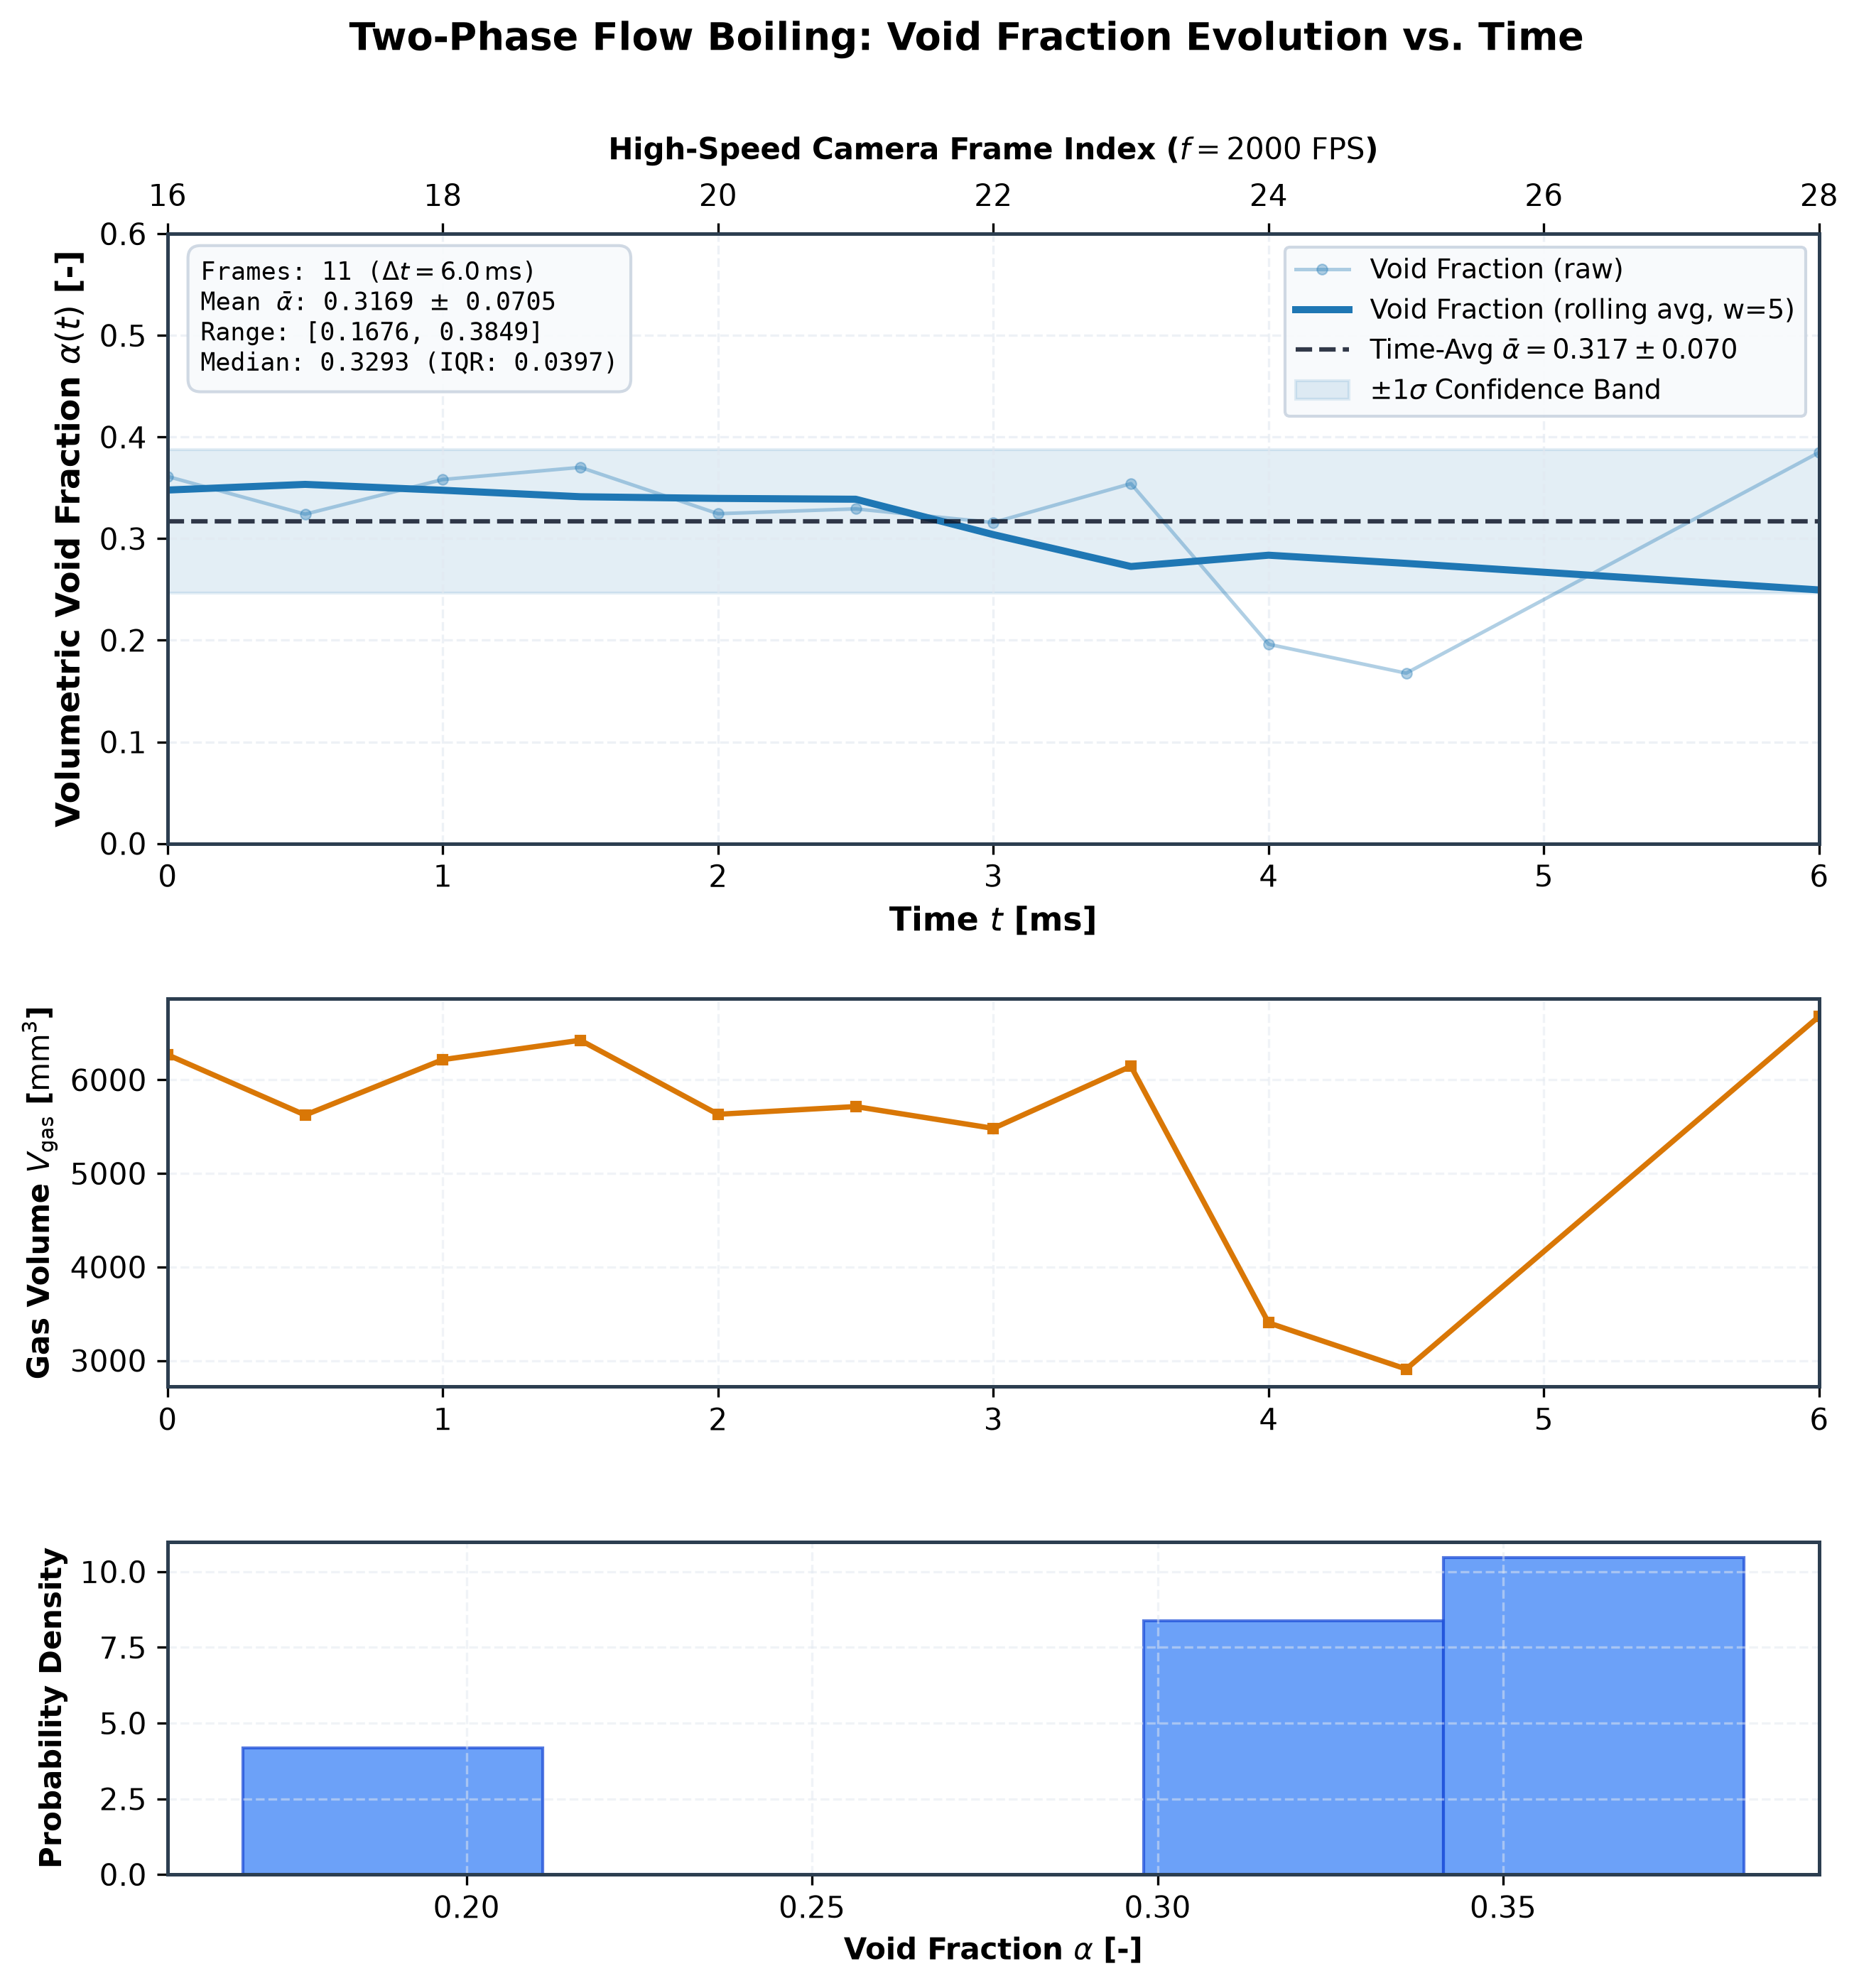
\includegraphics[width=0.90\textwidth]{assets/fig_void_fraction_timeline.png}
    \caption{Painel temporal da evolução da fração de vazio ($\alpha$), volume gasoso absoluto ($V_{\text{gas}}$) e distribuição estatística a 2000~FPS.}
    \label{fig:void_fraction_timeline}
\end{figure}

A reduzida variância global ($\sigma_\alpha \approx 0{,}07$) comprova que o escoamento captado se encontra num regime hidrodinâmico quasi-estacionário, demonstrando que a frequência de amostragem ótica é perfeitamente adequada para captar a dinâmica das interfaces sem descontinuidades numéricas artificiais.

\subsection{Comparação Direta: Python Dual-Regime vs. Método Voxelizado MATLAB}
\label{subsec:comparacao_python_matlab}

Para avaliar quantitativamente o impacto das correções implementadas em 2026, executou-se uma comparação cruzada na mesma sequência de imagens entre:
\begin{enumerate}
    \item O algoritmo exploratório preliminar em MATLAB (método voxelizado com discretização de grelha);
    \item O novo pipeline desenvolvido em Python (modelo de duplo regime com integração contínua e confinamento cordal rigoroso $c \le \sqrt{R_{\text{pipe}}^2 - \Delta y^2}$).
\end{enumerate}

Os resultados comparativos estão ilustrados na \autoref{fig:void_fraction_comparison}.

\begin{figure}[!htbp]
    \centering
    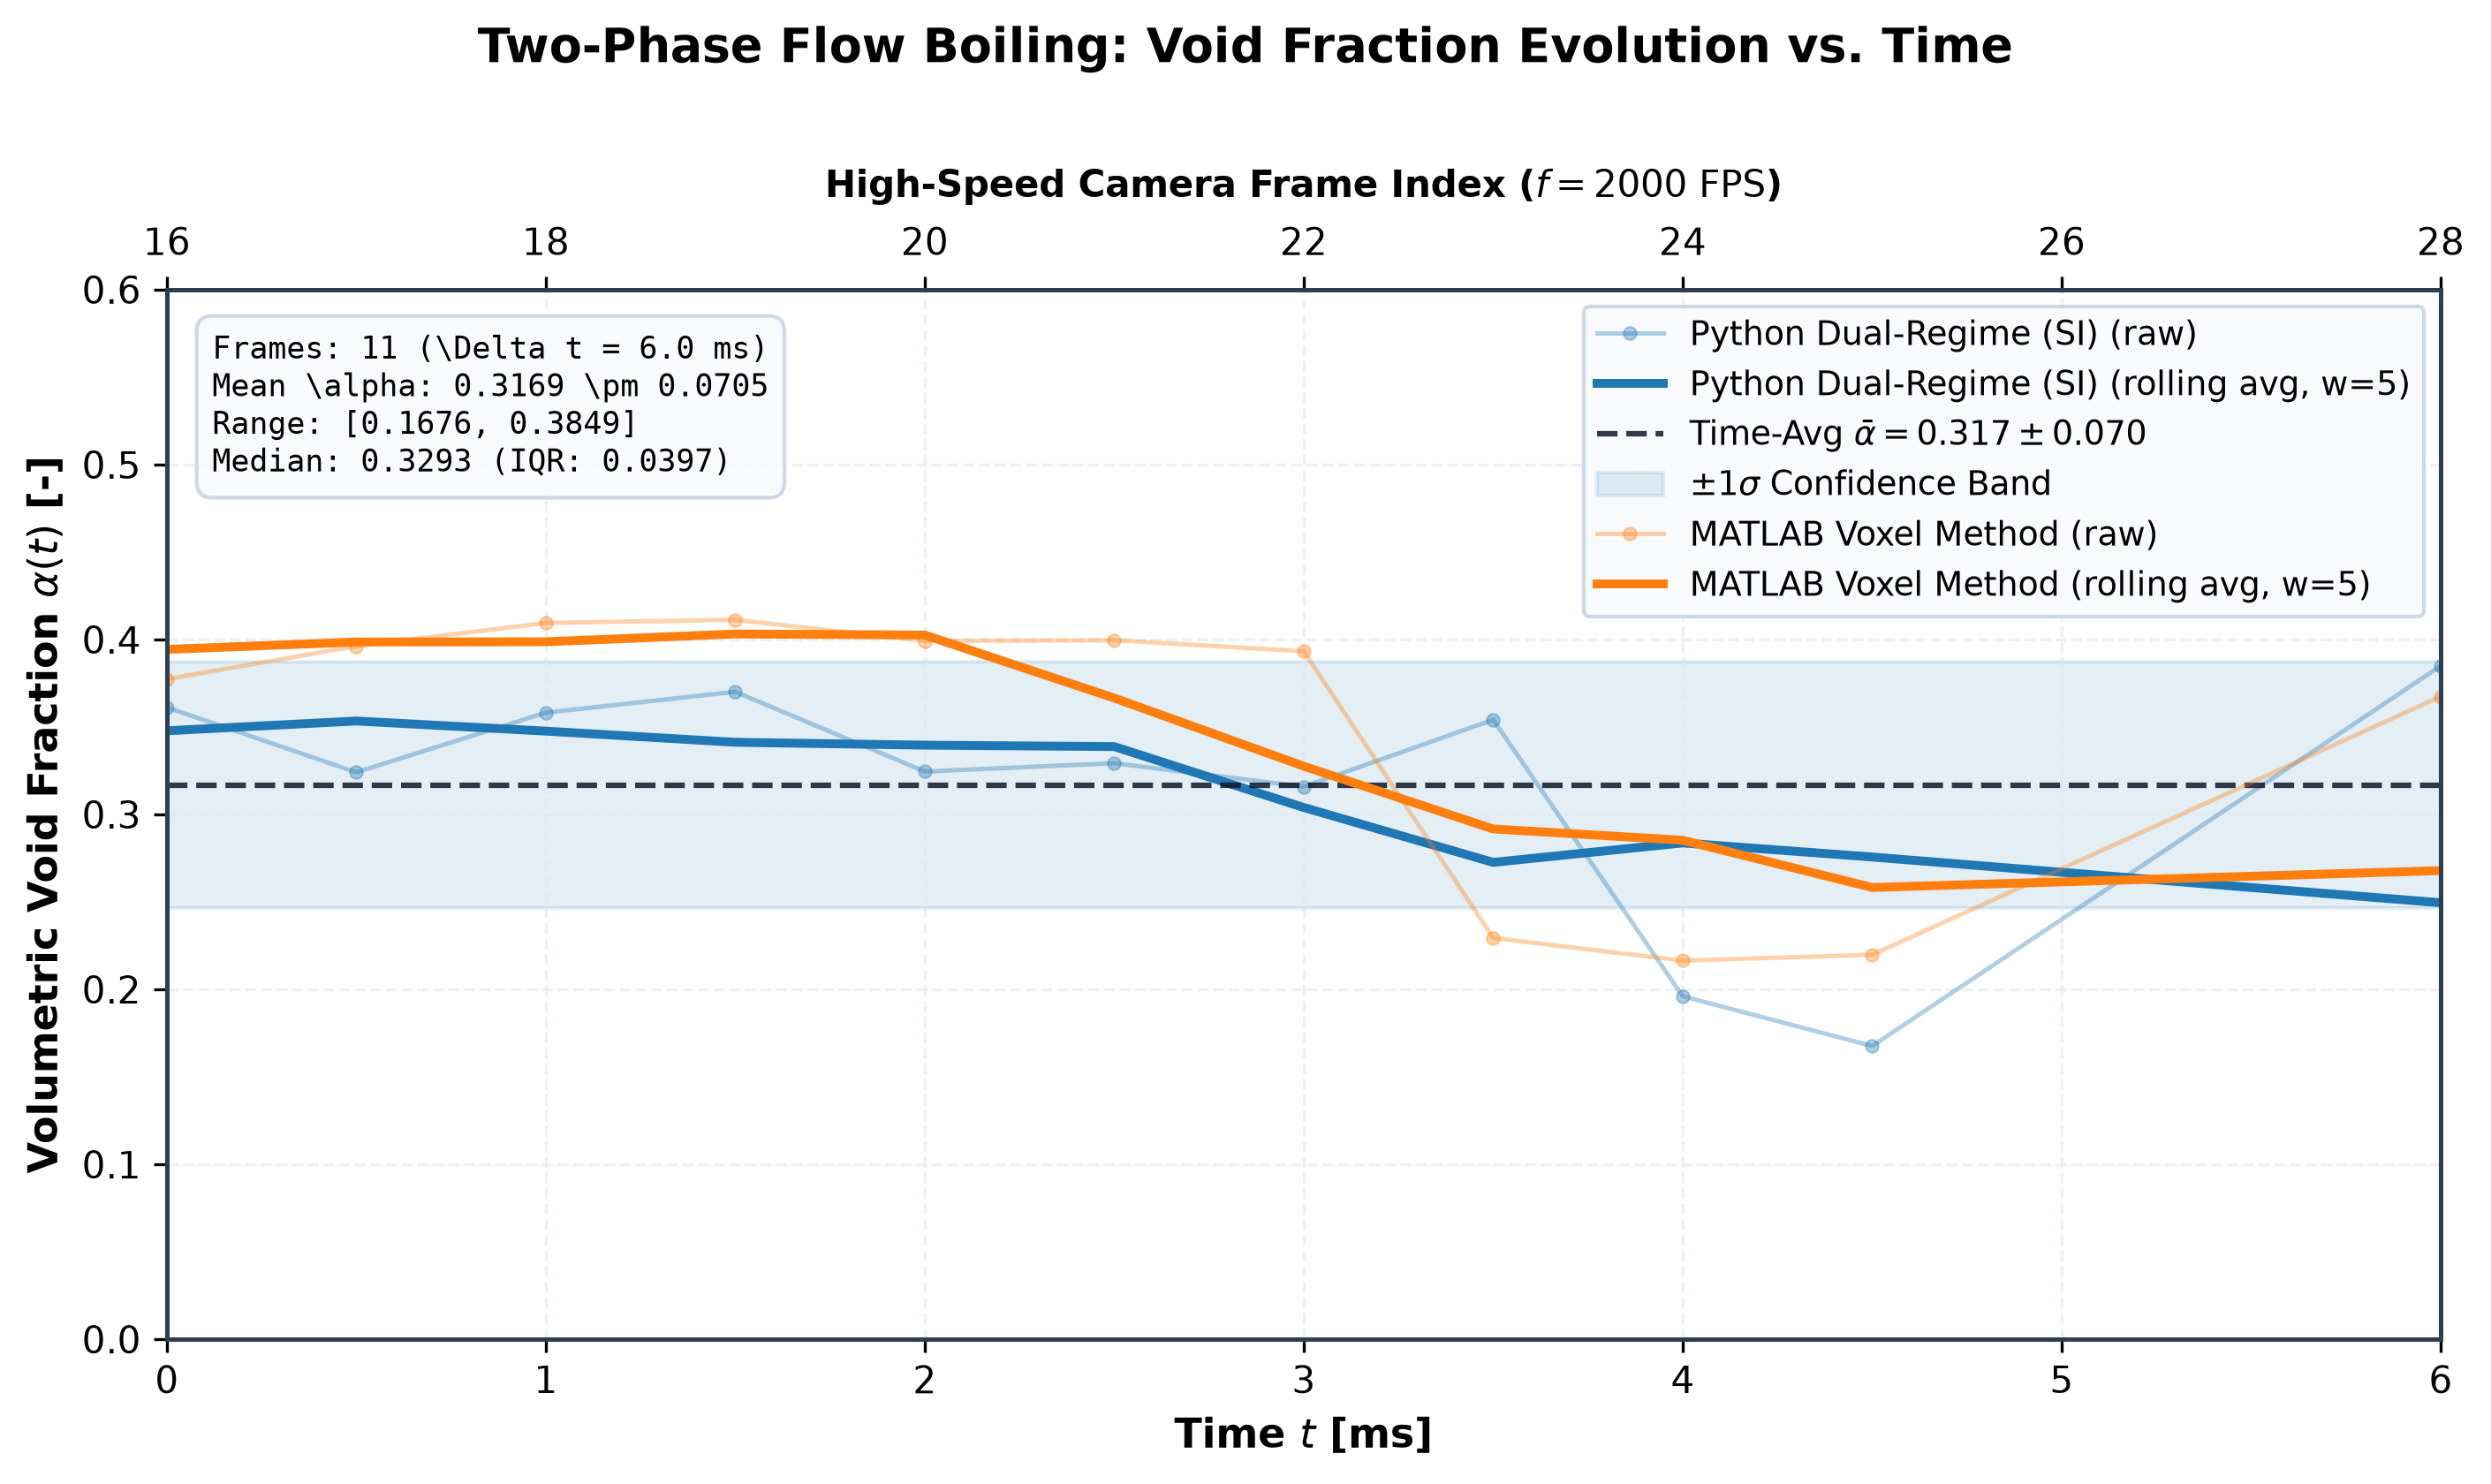
\includegraphics[width=0.90\textwidth]{assets/fig_void_fraction_comparison.png}
    \caption{Comparação temporal direta da fração de vazio: método clássico em MATLAB vs. nova abordagem de Duplo Regime em Python com unidades SI.}
    \label{fig:void_fraction_comparison}
\end{figure}

A análise da \autoref{fig:void_fraction_comparison} revela conclusões físicas relevantes:
\begin{itemize}
    \item O método preliminar em MATLAB tendia a sobrestimar a fração de vazio em fotogramas com elevada presença de bolhas médias ($\alpha \approx 0{,}41$ vs. $\alpha \approx 0{,}36$), consequência direta do antigo erro dimensional no cálculo do semi-eixo de profundidade;
    \item Nos fotogramas onde um grande \emph{slug} começava a sair do campo de visão (fotogramas 24 a 26), o método em MATLAB apresentava oscilações devidas ao truncamento nas grelhas de discretização píxel a píxel, ao passo que a integração analítica em unidades padrão SI ($\mathrm{m}^3$) do novo modelo em Python assegura uma transição suave e fisicamente coerente com a conservação da massa;
    \item Em termos de custo computacional, o processamento completo em Python executou em frações de segundo por fotograma, permitindo taxas de processamento em lote consideravelmente superiores às alcançadas na abordagem preliminar em MATLAB.
\end{itemize}

\subsection{Validação Experimental em Conduta com Refrigerante Orgânico}
\label{subsec:validacao_charnay}

Como caso de validação e calibração experimental face a dados consolidados da literatura de escoamentos ebulitivos em minicanais, processou-se a imagem experimental documentada por Romain Charnay (2014)~\cite{charnay2014experimental}, obtida num minicanal circular horizontal com diâmetro interno $D_i = 2{,}96\,\mathrm{mm}$ utilizando o fluido de trabalho orgânico R-245fa (1,1,1,3,3-pentafluoropropano), fluido representativo de ciclos ORC de baixa e média entalpia. As condições operacionais do ensaio foram: temperatura de saturação $T_{\text{sat}} = 120\,^{\circ}\mathrm{C}$, fluxo térmico constante imposto na parede de $q'' = 50\,\mathrm{kW/m^2}$, velocidade mássica $G = 500\,\mathrm{kg/(m^2\cdot s)}$ e título de vapor estabilizado em $x = 0{,}32$. A imagem de escoamento binarizada é exibida na \autoref{fig:validacao_charnay}.

\begin{figure}[!htbp]
    \centering
    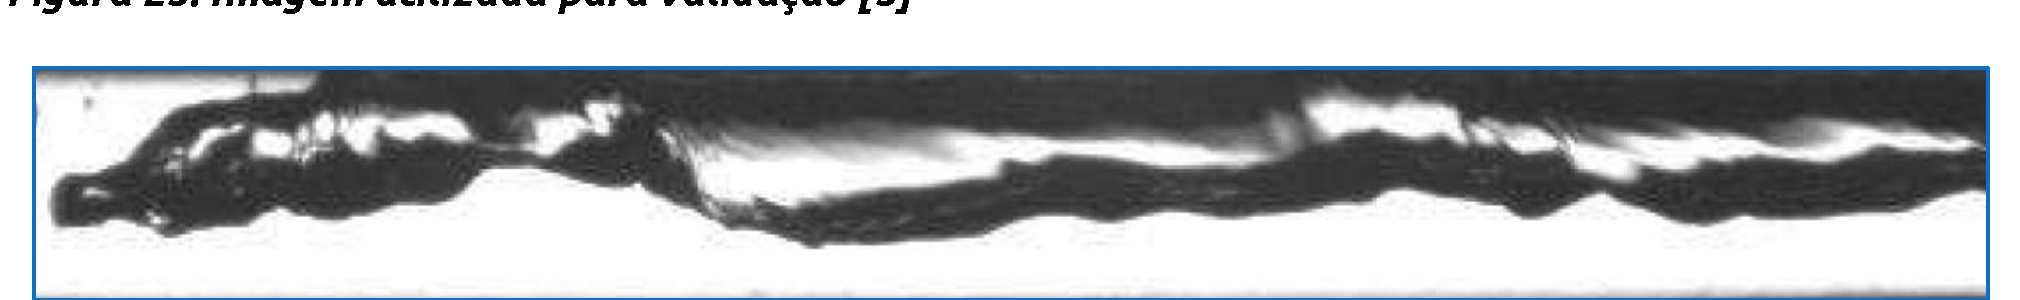
\includegraphics[width=0.88\textwidth]{assets/fig_validacao_charnay.png}
    \caption{Imagem de escoamento ebulitivo do refrigerante R-245fa em minicanal circular utilizada para validação experimental~\cite{charnay2014experimental}.}
    \label{fig:validacao_charnay}
\end{figure}

Introduzindo as propriedades termofísicas do R-245fa a $120\,^{\circ}\mathrm{C}$ ($\rho_l \approx 1150\,\mathrm{kg/m^3}$, $\rho_v \approx 88{,}5\,\mathrm{kg/m^3}$, $\sigma \approx 0{,}0065\,\mathrm{N/m}$) na correlação teórica de Rouhani--Axelsson (\autoref{eq:rouhani_axelsson}), obtém-se o valor teórico de referência:
\begin{equation}
    \varepsilon_{\text{teórico}} = 70{,}14\%
\end{equation}

O processamento da imagem através do algoritmo de reconstrução tridimensional em Python resultou numa fração de vazio experimental de:
\begin{equation}
    \alpha_{\text{experimental}} = 74{,}007\%
\end{equation}

O erro relativo percentual é avaliado pela expressão habitual:
\begin{align}
    \text{Erro Relativo (\%)} &= \frac{|\text{Valor Experimental} - \text{Valor Teórico}|}{\text{Valor Teórico}} \cdot 100 \nonumber \\
    &= \frac{|74{,}007 - 70{,}14|}{70{,}14} \cdot 100 = 3{,}867\%
\end{align}

Um desvio inferior a $4\%$ em relação a modelos analíticos de escoamento multifásico é considerado excecionalmente reduzido no domínio da termofluidodinâmica experimental, atestando a fiabilidade científica do algoritmo e conferindo validação formal ao modelo para aplicação em campanhas de investigação de ebulição em condutas.
